% Template PNSAC newsletter - Article
% Language: Latex
%

% Head

\title{North Star tail removal photographs}
%% \author{Drew Hodge}

\maketitle

%\end{multicols}

\begin{figure}[httb]
   \vspace{2em}
   \centering
   \includegraphics[scale=1.2]{"northstar tail remove 2018-2-X2-scaled".png}
%   \caption*{\small \em Scaffold erected next to North Star to support removal of the rudder and vertical stablizer.}
   \label{fig:stab-one}
\end{figure}

\begin{figure}[httb]
   \vspace{2em}
   \centering
   \includegraphics[scale=1.2]{"northstar tail remove 2018-4-X2-scaled".png}
%   \caption*{\small \em Scaffold erected next to North Star to support removal of the rudder and vertical stablizer.}
   \label{fig:stab-one}
\end{figure}

\begin{figure}[httb]
   \vspace{2em}
   \centering
   \includegraphics[scale=1.2]{"northstar tail remove 2018-15-X2-scaled".png}
%   \caption*{\small \em Scaffold erected next to North Star to support removal of the rudder and vertical stablizer.}
   \label{fig:stab-one}
\end{figure}

\begin{figure}[httb]
   \vspace{2em}
   \centering
   \includegraphics[scale=1.2]{"northstar tail remove 2018-16-X2-scaled".png}
%   \caption*{\small \em Scaffold erected next to North Star to support removal of the rudder and vertical stablizer.}
   \label{fig:stab-one}
\end{figure}

\begin{figure}[httb]
   \vspace{2em}
   \centering
   \includegraphics[scale=1.2]{"northstar tail remove 2018-3-X2-scaled".png}
%   \caption*{\small \em Scaffold erected next to North Star to support removal of the rudder and vertical stablizer.}
   \label{fig:stab-one}
\end{figure}

\begin{figure}[httb]
   \vspace{2em}
   \centering
   \includegraphics[scale=1.2]{"northstar tail remove 2018-19-X2-scaled".png}
%   \caption*{\small \em Scaffold erected next to North Star to support removal of the rudder and vertical stablizer.}
   \label{fig:stab-one}
\end{figure}

%\begin{figure}[ht!]
%   \vspace{2em}
%   \centering
%   %name of the graphic, without the path AND in EPS format:
%   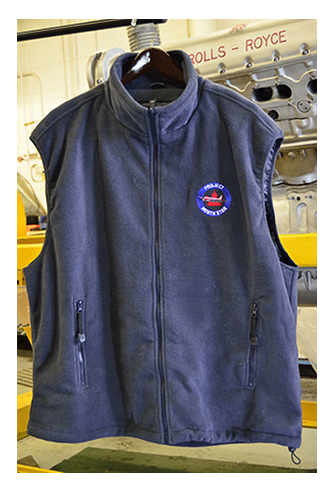
\includegraphics[scale=1.0]{fleece_YOW7578.eps}
%   %caption of the figure 
%   \caption*{\small \em PNSAC winter apparel}
%   %label of the figure, which has to correspond to \ref{}:
%   \label{fig:merchandise}
%\end{figure}

%\begin{enumerate}
%	\item "The Canadian North Star." This book and others referencing the North Star is available through Canavbooks ({\normalfont\color{blue}\texttt{\href{http://www.canavbooks.com}{www.canavbooks.com}}}).
%	\item "Short on Silence" is an article on CASM's North Star, included in the February 2016 edition of the British publication {\normalfont\color{blue}\texttt{\href{http://www.flypast.com/}{Fly Past Magazine}}}.
%	\item Models. There are only two metal models of the North Star left, and it is not presently intended to re-order. The models are for sale at CASM's gift shop.
%\end{enumerate}



\begin{footnotesize}
    \raggedleft PNSAC\\
\end{footnotesize}

%\begin{multicols}{2}

% End of text.

%%% Local Variables: 
%%% mode: latex
%%% TeX-master: main_document.tex
%%% End: 

